\documentclass[compress,12pt]{beamer}

\addtobeamertemplate{navigation symbols}{}{%
    \usebeamerfont{footline}%
    \usebeamercolor[fg]{footline}%
    \hspace{1em}%
    \insertframenumber/\inserttotalframenumber
}

\usetheme{Arguelles}

\title{Multiagent Reinforcement Learning for Traffic Signal Control}
%  \subtitle{Simple, typographic beamer theme}
\event{}
\date{Feb. 12, 2024}
\author{Kevyn Kelso}
\institute{University of Colorado at Colorado Springs}
\email{kkelso@uccs.edu}
\github{KevynKelso}

\begin{document}

\frame[plain]{\titlepage}

\Section{Introduction}

\begin{frame}[bg=arguelles.png]
      \frametitle{Table of Contents}
      \begin{itemize}
      \item Problem Introduction
      \item Problem Formulation within MDP paradigm
      \item Exploration of Existing Methods
      \item Proposed Method
      \item Performance Metrics
      \item Expected Challenges
      \end{itemize}
      % \texttt{\textbackslash frame[plain,bg=demo-background.jpg]\{\textbackslash titlepage\}}
\end{frame}

\begin{frame}[bg=arguelles.png]
      \frametitle{Problem Introduction}
      \begin{itemize}
      \item 12-55\% of total commute time is caused by signalized intersections \cite{ault2021reinforcement}.
      \item RL approaches suggest a 73\% decrease in that time by efficiently controlling traffic signals \cite{ault2021reinforcement}.
      \item This project aims to reproduce and improve upon existing RL methods.
      \end{itemize}
      % \texttt{\textbackslash frame[plain,bg=demo-background.jpg]\{\textbackslash titlepage\}}
\end{frame}


\Section{MDP}

\begin{frame}[bg=arguelles.png]
      \frametitle{Problem Formulation}
      \begin{itemize}
      \item Traffic Signal Control (TSC) is a Partially Observable Markov Decision Process (POMDP), meaning the agent does not have a full picture of the state\cite{Almeida2022MultiagentRL} \cite{DBLP:journals/corr/abs-2004-04778} \cite{choi1999environment}.
      \item Multiagent approaches introduce non-stationary dynamics meaning the state transition and reward probabilities are not static\cite{choi1999environment} \cite{10.3389/frai.2022.805823}.
      \item State aliasing occurs in POMDPs where the agent finds two states that are different to be the same, resulting in inappropriate actions. 
      \item Centralized approaches have the curse of dimensionality or require unfeasible infrastructure\cite{DBLP:journals/corr/abs-2004-04778} \cite{ault2021reinforcement}.
      \end{itemize}
      % \texttt{\textbackslash frame[plain,bg=demo-background.jpg]\{\textbackslash titlepage\}}
\end{frame}

\begin{frame}[bg=arguelles.png]
      \frametitle{State Space}
      \begin{itemize}
        \item Modeled as vector in \ref{eq:state_space}\cite{Almeida2022MultiagentRL}.
      \item Each time step \(t\) corresponds to five seconds of actual traffic dynamics.
      \item \(\rho_1\) and \(\rho_2\) are binary variables \(\rho_1, \rho_2 \in \{0, 1\}\) indicating the state of the intersection lights.
      \item \(g\) indicates if the light has been green for the minimum specified time.
      \item \(L\) is the list of all lanes with density \(\Delta_l\) which is the number of vehicles in each lane divided by the capacity of that lane.
      \item \(q_l\) is the number of queued vehicles in each lane \(l \in L\).
      \end{itemize}
      % \texttt{\textbackslash frame[plain,bg=demo-background.jpg]\{\textbackslash titlepage\}}

\begin{equation}
s_t = [\rho_1, \rho_2, g, \Delta_1, \ldots, \Delta_L, q_1, \ldots, q_L]
\label{eq:state_space}
\end{equation}

\end{frame}

\begin{frame}[bg=arguelles.png]
      \frametitle{Action Space}
      \begin{itemize}
      \item Agent can select an action to put the intersection into one of four modes \(a_t \in \{a_1, a_2, a_3, a_4\}\).
      \item To change the intersection into a different mode, a mandatory yellow phase $\phi$ precedes the mode change.
      \end{itemize}
      % \texttt{\textbackslash frame[plain,bg=demo-background.jpg]\{\textbackslash titlepage\}}

    \begin{figure}[htbp]
      \centering
      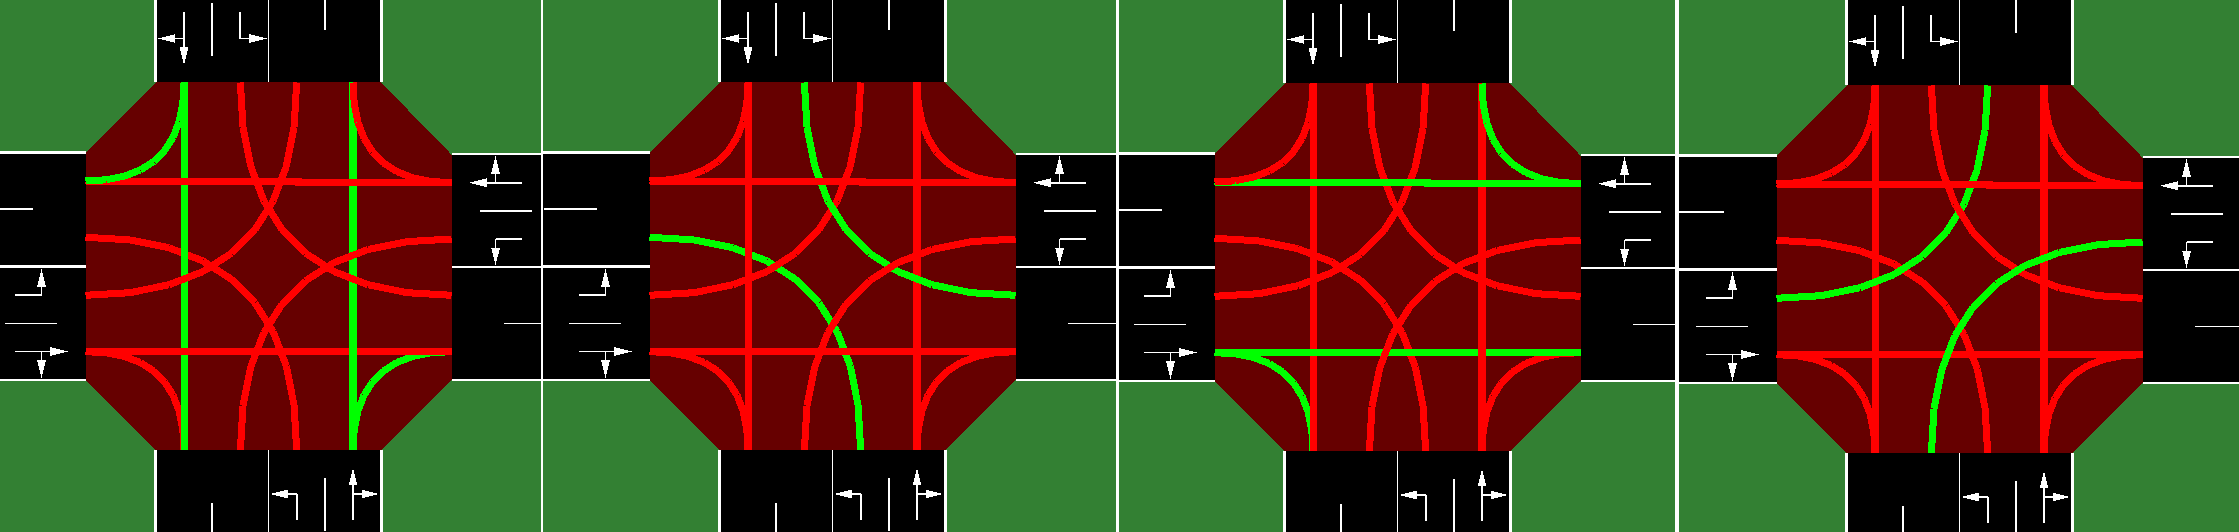
\includegraphics[width=0.8\linewidth]{actions.png}
      \caption{Traffic light modes}
      \label{fig:action_space}
    \end{figure}
\end{frame}

\begin{frame}[bg=arguelles.png]
      \frametitle{Reward Function}
      \begin{itemize}
      \item We use cumulative delay reward function \ref{eq:cumulative_delay} where \(D_t\) is the sum of all vehicles wait time \ref{eq:wait_time_sum}\cite{10.3389/frai.2022.805823}.
      \item \(V_t\) is the set of all vehicles in the simulation.
      \end{itemize}
      % \texttt{\textbackslash frame[plain,bg=demo-background.jpg]\{\textbackslash titlepage\}}

    \begin{equation}
    r_t = D_t - D_{t+1}
    \label{eq:cumulative_delay}
    \end{equation}

    \begin{equation}
    D_t = \sum_{v \in V_t} d_t^v
    \label{eq:wait_time_sum}
    \end{equation}
\end{frame}

\begin{frame}[bg=arguelles.png]
      \frametitle{Environment Simulator}
      \begin{itemize}
      \item Simulated Urban MObility (SUMO) will be used\cite{sumorl}.
      \item Widely accepted and used by the general transportation community\cite{ault2021reinforcement}.
      \item OpenAI PettingZoo API compatible\cite{terry2021pettingzoo}.
      \item Will use 4 x 4 grid scenario.
      \end{itemize}
      % \texttt{\textbackslash frame[plain,bg=demo-background.jpg]\{\textbackslash titlepage\}}

    \begin{figure}[htbp]
      \centering
      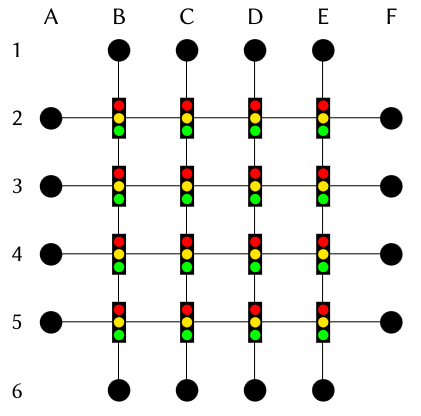
\includegraphics[width=0.4\linewidth]{4x4.png}
      \caption{4 x 4 intersection grid\cite{DBLP:journals/corr/abs-2004-04778}}
      \label{fig:intersection_grid}
    \end{figure}

\end{frame}

\begin{frame}[bg=logo.png]
\end{frame}

\Section{Methods}

\begin{frame}[bg=arguelles.png]
      \frametitle{Existing Methods}
      \begin{itemize}
      \item Traditional controllers use either fixed time, max pressure, or greedy\cite{ault2021reinforcement}\cite{Chen_Wei_Xu_Zheng_Yang_Xiong_Xu_Li_2020}.
      \item Independent Deep Q-Learning Networks (IDQN), Independent Proximal Policy Optimization (IPPO), MPLight (variant of DQN)\cite{Chen_Wei_Xu_Zheng_Yang_Xiong_Xu_Li_2020}, Feudal Multiagent Advantage Actor-Critic (FMA2C, MA2C)\cite{DBLP:journals/corr/abs-1903-04527}, State Action Reward State Action Lambda \(SARSA(\lambda)\), TD methods\cite{Reza2023}, Self Adaptive Systems (SAS), and ontology-based RL models\cite{Ghanadbashi2023}.
      \end{itemize}
      % \texttt{\textbackslash frame[plain,bg=demo-background.jpg]\{\textbackslash titlepage\}}

\end{frame}

\begin{frame}[bg=arguelles.png]
      \frametitle{Existing Methods}

    \begin{table}[H]
    \centering
    \small
    \begin{tabular}{lc}
    \hline
    \textbf{Method} & \textbf{Average Cumulative Delay (seconds)} \\ \hline
    Fixed Time      & 90.00\footnotemark[2]  \\
    Max Pressure    & 70.00\footnotemark[2]  \\
    Greedy          & 60.00\footnotemark[2]  \\
    IDQN            & 30.74                  \\
    IPPO            & 36.15                  \\
    MPLight         & 54.58                  \\
    MA2C            & 38.07\footnotemark[1]                  \\
    FMA2C           & 42.26                  \\
    \(SARSA(\lambda)\)           & 18.00\footnotemark[2]                  \\
    Ontology        & 17.00\footnotemark[2]                  \\ \hline
    \end{tabular}
    \caption{Average Delay Across All Scenarios}
    \label{tab:avg_delay}
    \end{table}
    \footnotetext[1]{Data was only collected in one scenario and may not reflect how the model performs in other scenarios.}
    \footnotetext[2]{Data was extracted from graphs.}
\end{frame}

\begin{frame}[bg=arguelles.png]
      \frametitle{Chosen Method}
      \begin{itemize}
      \item IDQN is the chosen approach to solve the TSC problem.
      \item IDQN is an off-policy, model-free RL method incorporating the idea of collecting experience tuples as the agent plays episodes\cite{DBLP:journals/corr/MnihKSGAWR13}.
      \item A deep neural network is used as a Q function approximator. Input is the state vector, output is Q values.
      \item Experience tuples used to train the deep neural network. This is known as experience replay.
      \item Actions are selected based on \(\epsilon\)-greedy algorithm where \(\epsilon\) is the probability the agent will choose a random action\cite{Mnih2015}.
      \item Higher values of \(\epsilon\) result in more exploration, while lower values result in more exploitation.
      \end{itemize}
      % \texttt{\textbackslash frame[plain,bg=demo-background.jpg]\{\textbackslash titlepage\}}
\end{frame}

\begin{frame}[bg=arguelles.png]
      \frametitle{Performance Metrics}
      \begin{itemize}
      \item REinforced Signal COntrol (RESCO) is a testbed and benchmark environment to help judge the performance of RL-based algorithms for TSC\cite{ault2021reinforcement}.
      \item Total wait time for each vehicle.
      \item Average delay per vehicle.
      \item Average number of stops per vehicle.
      \item Average queue length.
      \item Average trip time\cite{Reza2023}.
      \end{itemize}
      % \texttt{\textbackslash frame[plain,bg=demo-background.jpg]\{\textbackslash titlepage\}}
\end{frame}

\Section{Conclusion}

\begin{frame}[bg=arguelles.png]
      \frametitle{Expected Challenges}
      \begin{itemize}
      \item The non-stationary nature of multiagent RL problems is known to cause divergence problems due to the constantly changing dynamics.
      \item This can be somewhat mitigated by applying a scenario that is consistent across training, but the dynamics will still be changing due to the other agents' learning\cite{DBLP:journals/corr/abs-2004-04778}.
      \item Introducing context switches by changing the scenario, for example, making vehicles flow in waves to simulate rush hour is critical to designing a robust traffic system but will be out of the scope of the initial research goals.
      \end{itemize}
      % \texttt{\textbackslash frame[plain,bg=demo-background.jpg]\{\textbackslash titlepage\}}
\end{frame}

\begin{frame}[bg=arguelles.png]
      \frametitle{Timeline}

    \begin{table}[H]
    \centering
    \begin{tabular}{ll}
    \hline
    \textbf{Date} & \textbf{Milestone}             \\ \hline
    2/19 & 4x4 grid environment setup and working  \\
    2/26 & IDQN agents learning                    \\
    3/4  & Perform experiments and generate data   \\
    3/18 & Injected uncertainty scenarios          \\
    4/1  & Data compilation and writing            \\ \hline
    \end{tabular}
    \caption{Project Timeline}
    \label{tab:project_timeline}
    \end{table}

      % \texttt{\textbackslash frame[plain,bg=demo-background.jpg]\{\textbackslash titlepage\}}
\end{frame}

\begin{frame}[plain,standout]
      \centering
      Any questions? \\
      Thank you for listening!
      \vfill
    \begin{figure}[htbp]
      \centering
      \includegraphics[width=0.4\linewidth]{black_mountain_lion.jpg}
    \end{figure}
\end{frame}

\begin{frame}[allowframebreaks]
        \frametitle{References}
        \bibliographystyle{amsalpha}
        \bibliography{proposal.bib}
\end{frame}

\end{document}
